% ======================================================================
% §8  External validation: the Santiago instances
% ======================================================================
\FloatBarrier
\section{External validation: the Santiago instances}
\label{sec:santiago}

The predictions derived from the Fogo study (Section~\ref{sec:results})
were pre-registered before the Santiago data were processed.
Two independent instances from Santiago Island, Cape Verde, are evaluated
here: the whole island (S-T) and the southern region comprising the
concelhos of Praia, São Domingos, and Ribeira Grande de Santiago
($\approx395$\,km\textsuperscript{2}; S-N).
Both instances use the same weight-draw protocol and software pipeline
as the Fogo analysis (Section~\ref{sec:methods}), but were produced on
separate grids with fresh Pareto frontiers.
Results are reported at $\kappa=200$ unless noted; all bootstrap
confidence intervals use $B=2000$ draws and a \texttt{SeedSequence}
initialised at 20261104.

% ----------------------------------------------------------------------
\subsection{Instance descriptors}
\label{sec:santiago-instances}
% ----------------------------------------------------------------------

Table~\ref{tab:santiago-descriptors} compares the three instances on the
scale and difficulty measures that the predictions depend on.

\begin{table*}[!t]
\centering
\caption{Instance descriptors for Fogo (reference) and the two Santiago
  instances (S-T: whole island; S-N: southern region).
  $N_\text{cand}$: candidate sites before the spacing filter.
  $N_\text{adm}$: sites admitted after exclusion-zone removal.
  $N_\text{trios}$: feasible three-site portfolios satisfying~$d_\text{min}$.
  $\mathrm{TV}$, $\mathrm{TV}_B$, $\mathrm{TV}_W$: total variation,
  bottom-tercile variant, and criterion-weighted variant
  (Section~\ref{sec:lemmaconf}).
  $M_\text{eff} = 1/\!\sum_j w_j^2$ under nominal AHP weights.
  $p_\text{max}^c$: largest continuous point mass in the SAW/vec/opt
  $Q_2$ distribution at $\kappa=200$ (S5 testability criterion; see
  Section~\ref{sec:factorial}).
  $d_\text{min}$: enforced inter-site separation.
  Dashes: metric not computed for Fogo.}
\label{tab:santiago-descriptors}
\begin{tabular*}{\textwidth}{@{\extracolsep{\fill}}lrrr}
\toprule
Property                              & \textbf{Fogo}  & \textbf{S-T}                            & \textbf{S-N} \\
\midrule
$N_\text{cand}$                       & \Ncand         & \SantSTNcand                            & \SantSNNcand \\
$N_\text{adm}$                        & \FogoRefNadm   & \SantSTNadm                             & \SantSNNadm  \\
$N_\text{trios}$                      & \FogoRefNtrios & \SantSTNtrios                           & \SantSNNtrios \\[3pt]
$\mathrm{TV}$                         & \FogoRefTV     & \SantSTTV                               & \SantSNTV \\
$\mathrm{TV}_B$                       & \FogoRefTVB    & \SantSTTVB                              & \SantSNTVB \\
$\mathrm{TV}_W$                       & \FogoRefTVW    & \SantSTTVW                              & \SantSNTVW \\
$M_\text{eff}$                        & \FogoRefMeff   & \SantSTMeff                             & \SantSNMeff \\[3pt]
$p_\text{max}^c$                      & ---            & \SantSTSfivePerm                        & \SantSNSfivePerm \\
$d_\text{min}$ (m)                    & ---            & \SantSTSpacing                          & \SantSNSpacing \\
\bottomrule
\end{tabular*}
\end{table*}

S-T has more candidate sites and a substantially larger trio space than Fogo
($N_\text{trios}=\SantSTNtrios$ vs $\FogoRefNtrios$), but lower TV values
($\mathrm{TV}=\SantSTTV$ vs $\FogoRefTV$), indicating less within-criterion
variation and therefore smaller normalisation distortions.
S-N has a much smaller feasible space ($N_\text{trios}=\SantSNNtrios$) and
the lowest TV ($\SantSNTV$), while its higher $M_\text{eff}$ ($\SantSNMeff$
vs $\FogoRefMeff$ for Fogo) reflects more uniform nominal weights across
criteria.
The large $p_\text{max}^c$ of S-T ($\SantSTSfivePerm$) exceeds the S5
testability threshold, making the S5 prediction not evaluable on that
instance; S-N passes the criterion ($p_\text{max}^c = \SantSNSfivePerm$).

% ----------------------------------------------------------------------
\subsection{Prediction outcomes}
\label{sec:santiago-outcomes}
% ----------------------------------------------------------------------

Table~\ref{tab:santiago-predictions} summarises all sixteen prediction
outcomes.
For S5, S6, S7a, and S7b, the Fogo column shows the corresponding
reference value from Section~\ref{sec:results}; for all other rows it
gives the section where the Fogo result is reported.

\begin{table*}[!t]
\centering
\caption{Prediction outcomes for the two Santiago instances at
  $\kappa=200$.
  Results in brackets are 95\% bootstrap confidence intervals (pp).
  For K3 and K6, the summary statistic spans all six stochastic
  $\kappa$ values ($25$--$1000$).
  S4 specifies that K5 is purely descriptive; no confirmation
  criterion applies.
  Fogo column: reference value (S5--S7b) or section reference
  (all other rows) for the corresponding Fogo result.
  $\dagger$: not testable ($p_\text{max}^c=\SantSTSfivePerm>\text{threshold}$);
  see Table~\ref{tab:santiago-descriptors}.}
\label{tab:santiago-predictions}
\begin{tabular*}{\textwidth}{@{\extracolsep{\fill}}
    l
    >{\raggedright\arraybackslash}p{3.2cm}
    >{\raggedright\arraybackslash}p{2.4cm}
    >{\raggedright\arraybackslash}p{4.4cm}
    >{\raggedright\arraybackslash}p{4.4cm}}
\toprule
\textbf{Pred} & \textbf{Claim} & \textbf{Fogo} &
  \textbf{S-T} & \textbf{S-N} \\
\midrule
S0   & SAW/mm/opt $Q_2=100\%$
     & \S\ref{sec:base}
     & PASS (\SantSTSzeroN/500 draws)
     & PASS (\SantSNSzeroN/500 draws) \\[2pt]
S1   & mm $>$ vec on $Q_2$
     & \S\ref{sec:factorial}
     & $+\SantSTSoneDiff$\,pp [$\SantSTSoneCIlo$, $\SantSTSoneCIhi$]; confirmed
     & $+\SantSNSoneDiff$\,pp [$\SantSNSoneCIlo$, $\SantSNSoneCIhi$]; confirmed \\[2pt]
S2   & $Q_2(\text{opt}) > Q_2(\text{grd})$
     & \S\ref{sec:greedy}
     & absent: trios identical, $Q_2$ diff $= \SantSTStwoDiff$\,pp
       (\SantSTStwoSoloGrd{} vs \SantSTStwoSoloOpt{} exclusive draws)
     & opp.\ sign: $\SantSNStwoDiff$\,pp [$\SantSNStwoCIlo$, $\SantSNStwoCIhi$]
       (\SantSNStwoSoloGrd{} vs \SantSNStwoSoloOpt{} exclusive draws) \\[2pt]
S3a  & E1-W, E1-V both improve $Q_2$
     & \S\ref{sec:e1}
     & W: $\SantSTSthreeaEoneW$\%; V: $\SantSTSthreeaEoneV$\%; confirmed
     & W: $\SantSNSthreeaEoneW$\%; V: $\SantSNSthreeaEoneV$\%; confirmed \\[2pt]
S3b  & E1-V $<$ E1-W (regret)
     & \S\ref{sec:e1}
     & not confirmed: $+\SantSTSthreebDiff$\,pp
       ($\SantSTSthreebSoloV$ vs $\SantSTSthreebSoloW$; $p=\SantSTSthreebPval$)
     & confirmed: $\SantSNSthreebDiff$\,pp
       ($\SantSNSthreebSoloV$ vs $\SantSNSthreebSoloW$; $p=\SantSNSthreebPval$) \\[2pt]
S4   & K5 purely descriptive
     & \S\ref{sec:kappa}
     & \multicolumn{2}{l}{%
         \textit{Specification only; no confirmation criterion applies.}} \\[2pt]
S5   & SAW/vec/opt $Q_2$ high (if testable)
     & $\QtwovecOptimal$\%
     & not testable$^\dagger$
     & $\SantSNSfiveQvec$\%; confirmed \\[2pt]
S6   & $R_\text{grd} > R_\text{opt}$
     & \RegrSAWvecGrd{} vs \RegrSAWvecOpt\,pp
     & absent: trios identical in all 500 draws
     & $+\SantSNSsixDiff$\,pp [$\SantSNSsixCIlo$, $\SantSNSsixCIhi$]; confirmed \\[2pt]
S7a  & $R(E1\text{-}B) > 0$
     & \RegretEoneB\,pp; \RegretEoneBfracZero\%\ zeros
     & \SantSTSsvnaREoneB\,pp [\SantSTSsvnaCIlo, \SantSTSsvnaCIhi];
       \SantSTSsvnaFracZero\%\ zeros
     & \SantSNSsvnaREoneB\,pp [\SantSNSsvnaCIlo, \SantSNSsvnaCIhi];
       \SantSNSsvnaFracZero\%\ zeros \\[2pt]
S7b  & $R(E1\text{-}B) < R(E1\text{-}W)$
     & \RegretEoneB{} vs \RegretEoneW\,pp
     & $\Delta\in[\SantSTSsvnbCIlo,\,\SantSTSsvnbCIhi]$\,pp; confirmed
     & $\Delta\in[\SantSNSsvnbCIlo,\,\SantSNSsvnbCIhi]$\,pp; confirmed \\
\midrule
K1   & SAW/mm/opt $Q_2=100\%$ every draw
     & \S\ref{sec:base}
     & PASS (\SantSTKoneN/500)
     & PASS (\SantSNKoneN/500) \\[2pt]
K2   & E1-B/opt $Q_2=100\%$ at $\kappa=200$ and $\kappa\to\infty$
     & \S\ref{sec:e1}
     & PASS ($\kappa=200$: \SantSTKtwoN/500; $\kappa\to\infty$: \SantSTKtwoInfResult)
     & PASS ($\kappa=200$: \SantSNKtwoN/500; $\kappa\to\infty$: \SantSNKtwoInfResult) \\[2pt]
K3   & mm CI lower bound $>0$ for all $\kappa$
     & \S\ref{sec:kappa}
     & min CI lo $= \SantSTKthreeMinCIlo$\,pp; confirmed
     & min CI lo $= \SantSNKthreeMinCIlo$\,pp; confirmed \\[2pt]
K4   & detectable at some $\kappa$ (Holm)
     & \S\ref{sec:kappa}
     & $p_\text{Holm}=\SantSTKfourHolmP$; confirmed
     & $p_\text{Holm}=\SantSNKfourHolmP$; confirmed \\[2pt]
K5   & sign consistency (descriptive)
     & \S\ref{sec:kappa}
     & (a) null; (b) null
     & (a) same sign; (b) same sign \\[2pt]
K6   & agg.\ contrast $>0$ for all $\kappa$ (S-T);
       sign reversal with $\kappa$ (S-N)
     & \S\ref{sec:kappa}
     & \SantSTKsixKTwentyFive\,pp ($\kappa=25$) to
       \SantSTKsixKFourHundred\,pp ($\kappa=400$); no reversal
     & \SantSNKsixKFifty\,pp ($\kappa=50$),
       \SantSNKsixKHundred\,pp ($\kappa=100$); sign reversal \\
\bottomrule
\end{tabular*}
\end{table*}

\textbf{S2 and S6 jointly.}
On S-T, greedy assembly and optimal assembly select the same trio in every
weight draw at $\kappa=200$: the mean $Q_2$ difference is
$\SantSTStwoDiff$\,pp and $\SantSTStwoSoloGrd$ draws had exclusively greedy
trios on the frontier while $\SantSTStwoSoloOpt$ had exclusively optimal
trios (Table~\ref{tab:santiago-predictions}, S2).
The S6 regret gap is likewise $\SantSTSsixDiff$\,pp across all 500 draws.
Both absent effects reflect an instance where the criterion values under the
nominal weights are such that greedy assembly finds the optimal trio at
every stochastic realisation of the weights: a structural feature, not a
statistical result.
On S-N, both effects are present and in the predicted direction:
the $Q_2$ difference is $\SantSNStwoDiff$\,pp
(95\% CI [$\SantSNStwoCIlo$, $\SantSNStwoCIhi$], exclusive draws
$\SantSNStwoSoloGrd$ vs $\SantSNStwoSoloOpt$) and the regret gap
$R(\text{grd})-R(\text{opt}) = \SantSNSsixDiff$\,pp
(95\% CI [$\SantSNSsixCIlo$, $\SantSNSsixCIhi$]).

\textbf{S7a: zeros and magnitude.}
Both instances confirm that the E1-B intervention reduces regret relative to
the baseline, but the effect profiles differ.
On S-T, the fraction of draws where $R(E1\text{-}B)=0$ (the intervention
recovers the optimum exactly) is $\SantSTSsvnaFracZero$\%, closely matching
the Fogo reference ($\RegretEoneBfracZero$\%; Section~\ref{sec:e1}),
which suggests similar structural difficulty across the two instances.
On S-N, the confirmed mean regret of $\SantSNSsvnaREoneB$\,pp
(95\% CI [$\SantSNSsvnaCIlo$, $\SantSNSsvnaCIhi$]) is formally positive but
negligible in practice; the $\SantSNSsvnaFracZero$\% zero rate indicates
that the intervention trivially finds the optimum in most draws.

\textbf{S3b: opposite directions across instances.}
The pre-registered direction for S3b (E1-V outperforms E1-W) is confirmed
on S-N ($Q_2(E1\text{-}V)-Q_2(E1\text{-}W) = \SantSNSthreebDiff$\,pp;
$\SantSNSthreebSoloV$ vs $\SantSNSthreebSoloW$ exclusive-frontier draws;
exact binomial $p=\SantSNSthreebPval$)
but not on S-T ($+\SantSTSthreebDiff$\,pp in the opposite direction;
$\SantSTSthreebSoloV$ vs $\SantSTSthreebSoloW$;
McNemar $p=\SantSTSthreebPval$).
The two instances provide conflicting evidence on S3b, consistent with a
small and unstable effect that depends on properties of the specific
criterion distributions.

\textbf{K5 and K6.}
For S-T, K5 shows null sign agreement between $\kappa=1000$ and
$\kappa\to\infty$ on both (a) and (b); K6 is positive across all tested
$\kappa$ values ($\SantSTKsixKTwentyFive$\,pp at $\kappa=25$ to
$\SantSTKsixKFourHundred$\,pp at $\kappa=400$; Fig.~\ref{fig:kappa}).
For S-N, K5 shows same-sign agreement on both (a) and (b); K6 is positive at
$\kappa=50$ ($\SantSNKsixKFifty$\,pp, 95\% CI [$\SantSNKsixKFiftyLo$,
$\SantSNKsixKFiftyHi$]) and turns negative by $\kappa=100$
($\SantSNKsixKHundred$\,pp, 95\% CI [$\SantSNKsixKHundredLo$,
$\SantSNKsixKHundredHi$]), confirming the predicted sign reversal
(Fig.~\ref{fig:kappa}).
K5 and K6 are descriptive; no pre-registered confirmation criterion applies.

\begin{figure}[!t]
\centering
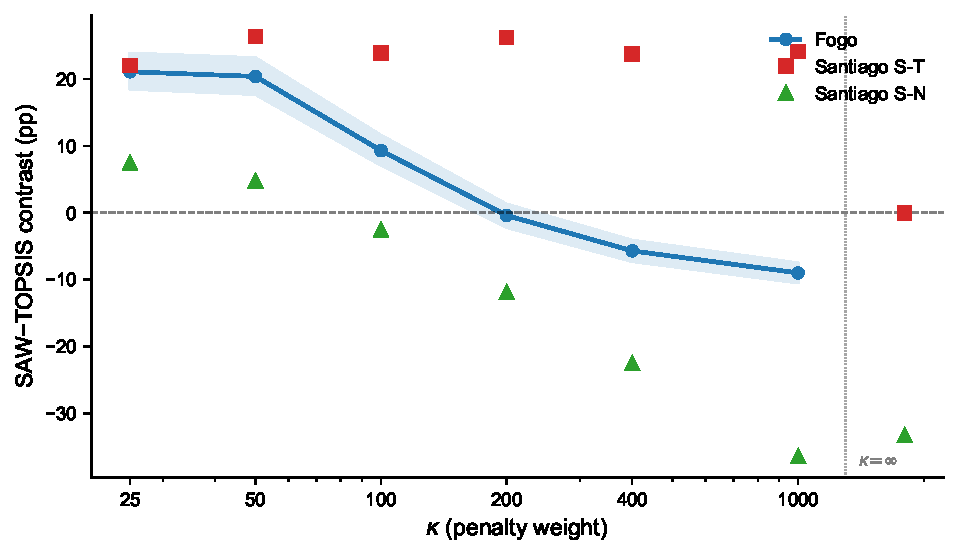
\includegraphics[width=\columnwidth]{figures/fig_kappa_santiago.pdf}
\caption{%
  Aggregation contrast (SAW minus TOPSIS, three informative cells,
  Section~\ref{sec:factorial}) as a function of weight concentration~$\kappa$
  for Fogo (filled circles), S-T (open squares), and S-N (open triangles).
  Shaded bands: descriptive 95\% bootstrap CIs ($B=2000$, percentile
  bootstrap; SeedSequence 20261104); CIs for the Santiago instances
  were computed after the evaluation was sealed and are not part of the
  pre-registered predictions.
  Grey band: equivalence margin $\pm\eqmargin=\pm2.5$\,pp (Fogo only;
  TOST from Section~\ref{sec:kappa}).
  Open diamond (Fogo, $\kappa=200$): the only Fogo interval that includes zero.
  Lower $\kappa$ means more dispersed weights.}
\label{fig:kappa}
\end{figure}
